\documentclass[12pt]{article}
\usepackage{minted}
\usepackage{graphics}
\renewcommand{\baselinestretch}{1.0}

\title{\textbf{Distribute System: Practical Work 1 }}
\vspace{10cm}
\author{\textbf{Group 5}}
\vspace{5cm}
\date{\textbf{January 2022}}

\begin{document}
\maketitle

\section{File transfer system}
\hspace{1.5cm}
 Files: \mintinline{text}{send.txt}, \mintinline{text}{receive.txt}
 
\vspace{0.5cm}
I failed to modify provided chat system but I succeed in transferring file with TCP.
\vspace{2cm}

\section{Design Protocol}
\begin{figure}
    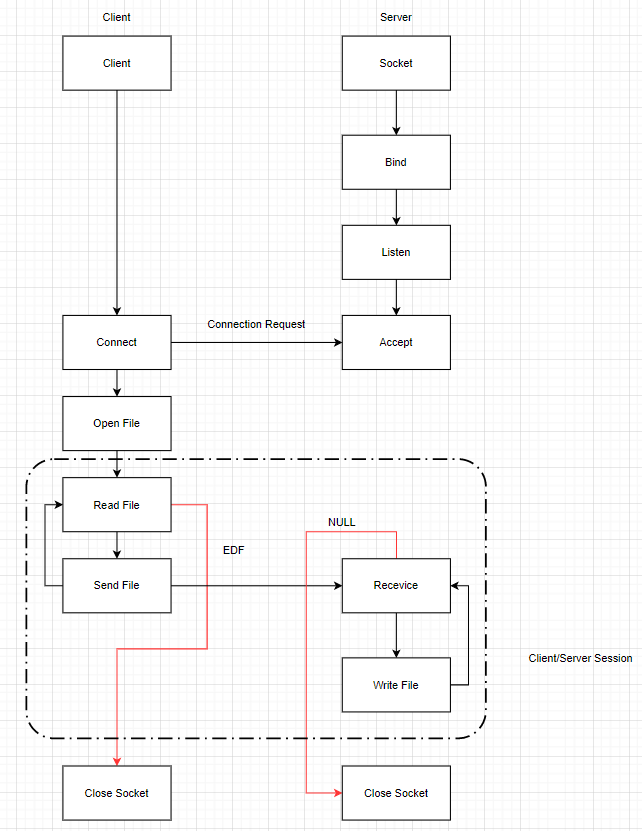
\includegraphics{Image/lab1.png}
    \caption{Protocol}
    \label{fig:my_label}
\end{figure}

\newpage
\section{Organizational system }
\vspace{1cm}
\begin{minted}{text}
                            +--------+
                            | Client |
                            +---+----+
                                |
                                |
                                |
                                | TCP /IP
                                |
                                |
                                v
                            +---+----+
                            | Server |
                            +--------+
\end{minted}
\vspace{0.5cm}
\begin{flushleft}
 The server only listen to one client. The client send data as chunks to the server. After receiving a chunk, the server writes to a file. After finishing writing the file, the server closes itself.
\end{flushleft}
\vspace{0.1cm}

\section{Implementation}
\hspace{0.5cm}
\textbf{ In \mintinline{text}{client.c}, the function to send file is implemented as followed.}
\hspace{1cm}
\begin{minted}{c}
#include <arpa/inet.h>
#include <netinet/in.h>
#include <stdio.h>
#include <stdlib.h>
#include <string.h>
#include <sys/socket.h>
#include <sys/types.h>
#include <unistd.h>
#define SIZE 1024
#define localhost "127.0.0.1"
#define port 3306
#define IP_PROTOCOL 0
#define NET_BUF_SIZE 32
#define cipherKey 'S'
#define sendrecvflag 0
void sending(FILE *document, int file){
  char buf[SIZE] = {0};
  while(fgets(buf, SIZE, document) != NULL) {
    if (send(file, buf, sizeof(buf), 0) == -1) {
      printf("Sending error.\n");
    }
    bzero(buf, SIZE);
  }
}
int main(int argc, char* argv[])
{
	int file;
	struct sockaddr_in addr_of_server;
	char *filename="test.txt";
	FILE* document;
	file = socket(AF_INET, SOCK_STREAM, IP_PROTOCOL);

	if (file < 0)
		printf("\nFile not received!!\n");
	else
		printf("\nFile %d received\n", file);

	int addrlen = sizeof(addr_of_server);
	addr_of_server.sin_family = AF_INET;
	addr_of_server.sin_port = port;
	addr_of_server.sin_addr.s_addr = inet_addr(localhost);
	if (connect(file, (struct sockaddr*)&addr_of_server, addrlen)==-1){
		printf("Socket error\n");
	}
	printf("\n---------Data Received---------\n");
	document = fopen(filename, "r");
  	if (document == NULL) {
    		printf("File reading error.\n");
  	}
  	sending(document, file);
  	printf("File sent successfully.\n");
  	close(file);
	return 0;
}


        
\end{minted}
\vspace{0.5cm}
\hspace{0.5cm}
 \textbf{In \mintinline{text}{servers.c}, the function to write file is implemented as followed}
 \hspace{1cm}
\begin{minted}{c}
#include <stdio.h>
#include <stdlib.h>
#include <string.h>
#include <arpa/inet.h>
#define SIZE 1024
#define localhost "127.0.0.1"
#define port 3306
#define IP_PROTOCOL 0
void create(int file){
  FILE *document;
  char *filename = "receives.txt";
  char bf[SIZE];
  document = fopen(filename, "w");
  while (1) {
    int n = recv(file, bf, SIZE, 0);
    if (n <= 0){
      break;
    }
    fprintf(document, "%s", bf);
    bzero(bf, SIZE);
  }
  return;
}
int main(int argc, char* argv[]){
  int file;
  int new_file;
  socklen_t size_of_address;
  char bf[SIZE];
  struct sockaddr_in ad, new_server_addr;
  size_of_address = sizeof(new_server_addr);
  file = socket(AF_INET, SOCK_STREAM, IP_PROTOCOL);
  if (file < 0)
        printf("\nFile not received!!\n");
    else
        printf("\nFile %d received\n", file);
  ad.sin_family = AF_INET;
  ad.sin_port = port;
  ad.sin_addr.s_addr = INADDR_ANY;
  if(bind(file, (struct sockaddr*)&ad, sizeof(ad))<0) {
    printf("Fail to bind\n");
  }
  printf("Binding successfully.\n");
  listen(file, 0);
  new_file = accept(file, (struct sockaddr*)&new_server_addr, &size_of_address);
  create(new_file);
  printf("Data written successfully.\n");
  return 0;
}
\end{minted}

\end{document}
